\documentclass[10pt,aspectratio=169]{beamer}
\usetheme{Madrid}
\usecolortheme{default}

\usepackage[utf8]{inputenc}
\usepackage[T1]{fontenc}
\usepackage{lmodern}
\usepackage{amsmath}
\usepackage{amssymb}
\usepackage{graphicx}
\usepackage{xcolor}
\usepackage{tikz}
\usepackage{adjustbox}
\usetikzlibrary{shapes.geometric, arrows, positioning}

\definecolor{entrygreen}{RGB}{0,150,0}
\definecolor{junctionblue}{RGB}{0,100,200}
\definecolor{linkgray}{RGB}{100,100,100}

\title[Simulation Victoria Island]{Simulation de Trafic - Victoria Island, Lagos}
\subtitle{Modèle ARZ Multi-Classe appliqué au Corridor Urbain}
\author{Présentation du Réseau et des Résultats}
\institute{Projet Alibi - Traffic Flow Simulation}
\date{\today}

\begin{document}

% --- Title Slide ---
\begin{frame}
    \titlepage
\end{frame}

% --- Table of Contents ---
\begin{frame}
    \frametitle{Plan de la Présentation}
    \tableofcontents
\end{frame}

% ============================================================
% SECTION 1: CONCEPTS DE BASE
% ============================================================
\section{Concepts de Base du Réseau}

\begin{frame}
    \frametitle{Qu'est-ce qu'un Réseau Routier ?}
    
    \begin{block}{Définition Simple}
        Un réseau routier, c'est comme un système de tuyaux où circule le trafic au lieu de l'eau.
    \end{block}
    
    \vspace{0.5cm}
    
    \begin{columns}[T]
        \begin{column}{0.5\textwidth}
            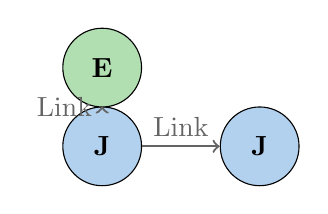
\begin{tikzpicture}[node distance=2cm]
                \node[circle, draw, fill=junctionblue!30, minimum size=1cm] (J1) {\textbf{J}};
                \node[circle, draw, fill=junctionblue!30, minimum size=1cm, right of=J1] (J2) {\textbf{J}};
                \node[circle, draw, fill=entrygreen!30, minimum size=1cm, above of=J1, yshift=-1cm] (E) {\textbf{E}};
                
                \draw[->, thick, linkgray] (E) -- node[left] {Link} (J1);
                \draw[->, thick, linkgray] (J1) -- node[above] {Link} (J2);
            \end{tikzpicture}
        \end{column}
        \begin{column}{0.5\textwidth}
            \begin{alertblock}{Les 3 Éléments Clés}
                \begin{itemize}
                    \item \textcolor{junctionblue}{\textbf{Jonction (J)}} : Point de rencontre
                    \item \textcolor{entrygreen}{\textbf{Entrée (E)}} : Arrivée de trafic
                    \item \textcolor{linkgray}{\textbf{Link}} : Route qui relie
                \end{itemize}
            \end{alertblock}
        \end{column}
    \end{columns}
\end{frame}

\begin{frame}
    \frametitle{C'est quoi une Jonction ?}
    
    \begin{block}{Définition}
        Une \textbf{jonction} est un point où plusieurs routes se rencontrent. C'est comme un carrefour ou une intersection.
    \end{block}
    
    \vspace{0.3cm}
    
    \begin{columns}[T]
        \begin{column}{0.5\textwidth}
            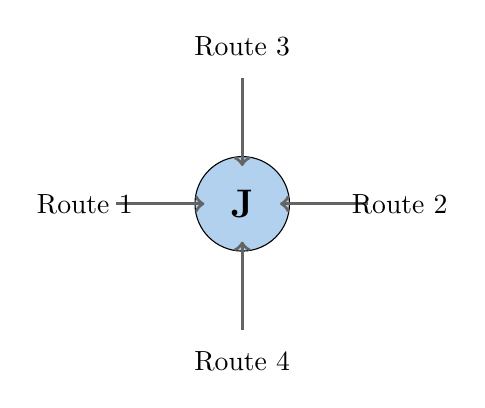
\begin{tikzpicture}[scale=0.8]
                % Jonction centrale
                \node[circle, draw, fill=junctionblue!30, minimum size=1.2cm] (center) at (0,0) {\Large\textbf{J}};
                
                % 4 routes qui arrivent
                \draw[->, very thick, linkgray] (-2,0) -- (-0.6,0);
                \draw[->, very thick, linkgray] (2,0) -- (0.6,0);
                \draw[->, very thick, linkgray] (0,2) -- (0,0.6);
                \draw[->, very thick, linkgray] (0,-2) -- (0,-0.6);
                
                \node at (-2.5, 0) {Route 1};
                \node at (2.5, 0) {Route 2};
                \node at (0, 2.5) {Route 3};
                \node at (0, -2.5) {Route 4};
            \end{tikzpicture}
        \end{column}
        \begin{column}{0.5\textwidth}
            \begin{exampleblock}{Rôle de la Jonction}
                \begin{itemize}
                    \item Collecte le trafic de plusieurs routes
                    \item Redistribue vers d'autres routes
                    \item Peut créer des embouteillages si surchargée
                \end{itemize}
            \end{exampleblock}
            
            \begin{alertblock}{Dans Victoria Island}
                60 jonctions coordonnent le trafic sur 70 routes !
            \end{alertblock}
        \end{column}
    \end{columns}
\end{frame}

\begin{frame}
    \frametitle{C'est quoi une Entrée (Entry) ?}
    
    \begin{block}{Définition}
        Une \textbf{entrée} est un point où les véhicules arrivent dans le réseau. C'est la "source" du trafic.
    \end{block}
    
    \vspace{0.3cm}
    
    \begin{columns}[T]
        \begin{column}{0.5\textwidth}
            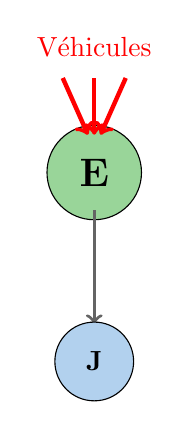
\begin{tikzpicture}[scale=0.8]
                % Entrée
                \node[circle, draw, fill=entrygreen!40, minimum size=1.2cm] (entry) at (0,2) {\Large\textbf{E}};
                
                % Flèche de trafic entrant
                \draw[->, ultra thick, red] (-0.5,3.5) -- (-0.1,2.6);
                \draw[->, ultra thick, red] (0,3.5) -- (0,2.6);
                \draw[->, ultra thick, red] (0.5,3.5) -- (0.1,2.6);
                
                \node at (0, 4) {\textcolor{red}{Véhicules}};
                
                % Link vers jonction
                \draw[->, very thick, linkgray] (0, 1.4) -- (0, -0.4);
                
                % Jonction
                \node[circle, draw, fill=junctionblue!30, minimum size=1cm] (junc) at (0,-1) {\textbf{J}};
            \end{tikzpicture}
        \end{column}
        \begin{column}{0.5\textwidth}
            \begin{exampleblock}{Caractéristiques d'une Entrée}
                \begin{itemize}
                    \item Injecte un flux constant de véhicules
                    \item Densité initiale : 30 véh/km
                    \item Vitesse initiale : 40 km/h
                \end{itemize}
            \end{exampleblock}
            
            \begin{alertblock}{Analogie}
                C'est comme un robinet qui verse de l'eau (véhicules) dans le réseau de tuyaux (routes).
            \end{alertblock}
        \end{column}
    \end{columns}
\end{frame}

\begin{frame}
    \frametitle{C'est quoi un Link (Tronçon de Route) ?}
    
    \begin{block}{Définition}
        Un \textbf{link} est un segment de route qui relie deux jonctions. C'est là où circulent les véhicules.
    \end{block}
    
    \vspace{0.3cm}
    
    \begin{columns}[T]
        \begin{column}{0.5\textwidth}
            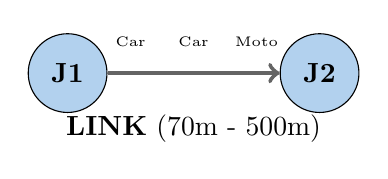
\begin{tikzpicture}[scale=0.8]
                % Deux jonctions
                \node[circle, draw, fill=junctionblue!30, minimum size=1cm] (J1) at (0,0) {\textbf{J1}};
                \node[circle, draw, fill=junctionblue!30, minimum size=1cm] (J2) at (4,0) {\textbf{J2}};
                
                % Link avec trafic
                \draw[->, ultra thick, linkgray] (J1) -- (J2);
                
                % Véhicules sur le link (symboles texte)
                \node at (1, 0.5) {\tiny Car};
                \node at (2, 0.5) {\tiny Car};
                \node at (3, 0.5) {\tiny Moto};
                
                \node[below] at (2, -0.5) {\textbf{LINK} (70m - 500m)};
            \end{tikzpicture}
        \end{column}
        \begin{column}{0.5\textwidth}
            \begin{exampleblock}{Propriétés d'un Link}
                \begin{itemize}
                    \item \textbf{Longueur} : Distance entre les jonctions
                    \item \textbf{Capacité} : Nombre max de véhicules
                    \item \textbf{Vitesse libre} : Vitesse sans embouteillage (50 km/h)
                \end{itemize}
            \end{exampleblock}
            
            \begin{alertblock}{Dans Victoria Island}
                70 links de longueurs variables (70m à 500m)
            \end{alertblock}
        \end{column}
    \end{columns}
\end{frame}

% ============================================================
% SECTION 2: LE RÉSEAU VICTORIA ISLAND
% ============================================================
\section{Le Réseau Victoria Island}

\begin{frame}
    \frametitle{Victoria Island : Vue d'Ensemble}
    
    \begin{block}{Localisation}
        Victoria Island est un quartier d'affaires très fréquenté de Lagos, Nigeria. C'est une zone avec beaucoup de circulation automobile et de motos.
    \end{block}
    
    \vspace{0.3cm}
    
    \begin{columns}[T]
        \begin{column}{0.5\textwidth}
            \begin{alertblock}{Statistiques du Réseau}
                \begin{itemize}
                    \item \textbf{60 jonctions} (intersections)
                    \item \textbf{70 links} (segments de route)
                    \item \textbf{2 classes de véhicules} :
                    \begin{itemize}
                        \item Motos (rapides, agiles)
                        \item Voitures (plus lentes, plus larges)
                    \end{itemize}
                \end{itemize}
            \end{alertblock}
        \end{column}
        \begin{column}{0.5\textwidth}
            \begin{exampleblock}{Caractéristiques Urbaines}
                \begin{itemize}
                    \item Trafic dense aux heures de pointe
                    \item Mix motos/voitures typique de Lagos
                    \item Routes de longueurs variées
                    \item Points d'entrée multiples
                \end{itemize}
            \end{exampleblock}
        \end{column}
    \end{columns}
    
    \vspace{0.3cm}
    \centering
    \textit{Objectif : Simuler 2 minutes de trafic réel sur ce réseau}
\end{frame}

\begin{frame}
    \frametitle{Configuration de la Simulation}
    
    \begin{block}{Paramètres Initiaux du Trafic}
        \begin{tabular}{lcc}
            \textbf{Paramètre} & \textbf{Valeur} & \textbf{Signification} \\
            \hline
            Densité de base & 20 véh/km & Trafic léger au départ \\
            Vitesse de base & 50 km/h & Circulation fluide \\
            Densité aux entrées & 30 véh/km & Plus de véhicules arrivent \\
            Vitesse aux entrées & 40 km/h & Légèrement ralentis \\
            \hline
        \end{tabular}
    \end{block}
    
    \vspace{0.3cm}
    
    \begin{columns}[T]
        \begin{column}{0.5\textwidth}
            \begin{exampleblock}{Durée de Simulation}
                \begin{itemize}
                    \item \textbf{Temps total} : 120 secondes (2 minutes)
                    \item \textbf{Snapshots} : Toutes les 2 secondes
                    \item \textbf{Total de frames} : 61 images
                \end{itemize}
            \end{exampleblock}
        \end{column}
        \begin{column}{0.5\textwidth}
            \begin{alertblock}{Résolution Spatiale}
                \begin{itemize}
                    \item \textbf{Maillage} : 10 cellules par 100m
                    \item Précision fine pour capturer les ondes de trafic
                \end{itemize}
            \end{alertblock}
        \end{column}
    \end{columns}
\end{frame}

% ============================================================
% SECTION 3: LES ÉQUATIONS PHYSIQUES
% ============================================================
\section{Comment ça Marche ? (Les Équations)}

\begin{frame}
    \frametitle{Le Modèle Physique : ARZ Multi-Classe}
    
    \begin{block}{Principe de Base}
        Le modèle ARZ calcule comment les véhicules se déplacent et s'influencent mutuellement sur chaque link.
    \end{block}
    
    \vspace{0.3cm}
    
    \textbf{Pour chaque classe de véhicule (motos \texttt{m}, voitures \texttt{c}), on calcule :}
    
    \begin{align*}
        \frac{\partial \rho}{\partial t} + \frac{\partial (\rho v)}{\partial x} &= 0 && \text{\small (Conservation : les véhicules ne disparaissent pas)} \\
        \frac{\partial w}{\partial t} + v \frac{\partial w}{\partial x} &= \frac{V_e(\rho) - v}{\tau} && \text{\small (Relaxation vers vitesse d'équilibre)}
    \end{align*}
    
    \vspace{0.3cm}
    
    \begin{alertblock}{Variables Physiques}
        \begin{itemize}
            \item $\rho$ : \textbf{Densité} (nombre de véhicules par km)
            \item $v$ : \textbf{Vitesse} (km/h)
            \item $w$ : Variable de "moment" (technique mathématique)
            \item $V_e$ : Vitesse d'équilibre que les conducteurs visent
        \end{itemize}
    \end{alertblock}
\end{frame}

\begin{frame}
    \frametitle{La "Pression" du Trafic : Comment les Véhicules se Gênent}
    
    \begin{block}{Concept Clé : La Pression $p(\rho)$}
        Plus il y a de véhicules (densité élevée), plus ils se gênent mutuellement, créant une "pression" qui ralentit tout le monde.
    \end{block}
    
    \vspace{0.3cm}
    
    \textbf{Formule mathématique :}
    $$ p(\rho) = K \left( \frac{\rho_{eff}}{\rho_{jam}} \right)^\gamma $$
    
    \vspace{0.3cm}
    
    \begin{columns}[T]
        \begin{column}{0.5\textwidth}
            \begin{exampleblock}{Pour les Motos}
                $$ \rho_{eff,moto} = \rho_{moto} + \alpha \cdot \rho_{voiture} $$
                \small Les motos sont \textbf{moins gênées} par les voitures ($\alpha < 1$) car elles peuvent se faufiler.
            \end{exampleblock}
        \end{column}
        \begin{column}{0.5\textwidth}
            \begin{exampleblock}{Pour les Voitures}
                $$ \rho_{eff,voiture} = \rho_{moto} + \rho_{voiture} $$
                \small Les voitures sont \textbf{gênées pareillement} par motos et voitures.
            \end{exampleblock}
        \end{column}
    \end{columns}
    
    \vspace{0.3cm}
    
    \begin{alertblock}{Impact sur la Vitesse}
        $$ v = w - p(\rho) \quad \Rightarrow \quad \text{Plus $p$ est grand, plus $v$ diminue !}$$
    \end{alertblock}
\end{frame}

\begin{frame}
    \frametitle{Configuration Appliquée : Valeurs Numériques}
    
    \begin{block}{Paramètres du Modèle ARZ}
        Ces valeurs définissent le comportement physique du trafic dans notre simulation.
    \end{block}
    
    \vspace{0.3cm}
    
    \begin{columns}[T]
        \begin{column}{0.5\textwidth}
            \begin{exampleblock}{Motos}
                \begin{itemize}
                    \item $\rho_{jam,m} = 180$ véh/km \\
                    \small (Capacité max : embouteillage)
                    \item $V_{free,m} = 60$ km/h \\
                    \small (Vitesse libre)
                    \item $\tau_m = 10$ s \\
                    \small (Temps de réaction)
                    \item $K_m, \gamma_m$ : Coefficients de pression
                \end{itemize}
            \end{exampleblock}
        \end{column}
        \begin{column}{0.5\textwidth}
            \begin{exampleblock}{Voitures}
                \begin{itemize}
                    \item $\rho_{jam,c} = 150$ véh/km \\
                    \small (Capacité max)
                    \item $V_{free,c} = 50$ km/h \\
                    \small (Vitesse libre, < motos)
                    \item $\tau_c = 12$ s \\
                    \small (Réaction plus lente)
                    \item $K_c, \gamma_c$ : Coefficients de pression
                \end{itemize}
            \end{exampleblock}
        \end{column}
    \end{columns}
    
    \vspace{0.3cm}
    
    \begin{alertblock}{Impact Attendu}
        Les motos devraient circuler plus vite et se faufiler, tandis que les voitures forment des files plus denses.
    \end{alertblock}
\end{frame}

% ============================================================
% SECTION 4: ANALYSE DES RÉSULTATS
% ============================================================
\section{Analyse des Résultats de Simulation}

\begin{frame}
    \frametitle{Comprendre les Couleurs de l'Animation}
    
    \begin{block}{Code Couleur : Vitesse Moyenne sur chaque Link}
        Les couleurs indiquent à quelle vitesse circulent les véhicules. 41 nuances pour une précision maximale !
    \end{block}
    
    \vspace{0.3cm}
    
    \begin{center}
        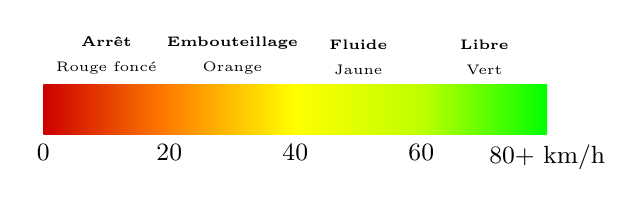
\begin{tikzpicture}[scale=0.8]
            % Barre de gradient
            \shade[left color=red!80!black, right color=yellow, middle color=orange] 
                (0,0) rectangle (4,0.8);
            \shade[left color=yellow, right color=green, middle color=lime] 
                (4,0) rectangle (8,0.8);
                
            % Labels
            \node[below] at (0,0) {\small 0};
            \node[below] at (2,0) {\small 20};
            \node[below] at (4,0) {\small 40};
            \node[below] at (6,0) {\small 60};
            \node[below] at (8,0) {\small 80+ km/h};
            
            % Descriptions
            \node[above, align=center] at (1, 0.8) {\tiny\textbf{Arrêt}\\[-0.1cm]\tiny Rouge foncé};
            \node[above, align=center] at (3, 0.8) {\tiny\textbf{Embouteillage}\\[-0.1cm]\tiny Orange};
            \node[above, align=center] at (5, 0.8) {\tiny\textbf{Fluide}\\[-0.1cm]\tiny Jaune};
            \node[above, align=center] at (7, 0.8) {\tiny\textbf{Libre}\\[-0.1cm]\tiny Vert};
        \end{tikzpicture}
    \end{center}
    
    \vspace{0.5cm}
    
    \begin{columns}[T]
        \begin{column}{0.5\textwidth}
            \begin{alertblock}{Rouge (0-10 km/h)}
                Presque arrêté - Embouteillage sévère
            \end{alertblock}
            \begin{exampleblock}{Orange (10-30 km/h)}
                Congestion - Trafic lent
            \end{exampleblock}
        \end{column}
        \begin{column}{0.5\textwidth}
            \begin{exampleblock}{Jaune (30-50 km/h)}
                Circulation correcte - Quelques ralentissements
            \end{exampleblock}
            \begin{alertblock}{Vert (50-80+ km/h)}
                Fluidité - Circulation libre
            \end{alertblock}
        \end{column}
    \end{columns}
\end{frame}

\begin{frame}
    \frametitle{Snapshot 1 : t = 0s (État Initial)}
    
    \begin{block}{Situation au Départ}
        Le réseau commence avec un trafic léger et une circulation fluide partout.
    \end{block}
    
    \vspace{0.3cm}
    
    \begin{columns}[T]
        \begin{column}{0.5\textwidth}
            \begin{exampleblock}{Observations Visuelles}
                \begin{itemize}
                    \item \textcolor{green}{\textbf{Couleur dominante : Vert/Jaune}}
                    \item Toutes les routes sont dégagées
                    \item Vitesses proches de la vitesse libre (50 km/h)
                    \item Densité faible : 20 véh/km
                \end{itemize}
            \end{exampleblock}
        \end{column}
        \begin{column}{0.5\textwidth}
            \begin{alertblock}{Ce qui se Passe}
                \begin{itemize}
                    \item Les véhicules commencent leur trajet
                    \item Pas encore d'interaction forte
                    \item Les entrées injectent du trafic (30 véh/km)
                    \item C'est le "calme avant la tempête"
                \end{itemize}
            \end{alertblock}
        \end{column}
    \end{columns}
    
    \vspace{0.3cm}
    
    \begin{center}
        \textit{\small (Regardez la figure network\_snapshots.png, panneau 1)}
    \end{center}
\end{frame}

\begin{frame}
    \frametitle{Snapshot 2 : t = 24s (Début de Congestion)}
    
    \begin{block}{Évolution du Trafic}
        Après 24 secondes, les premiers signes de congestion apparaissent.
    \end{block}
    
    \vspace{0.3cm}
    
    \begin{columns}[T]
        \begin{column}{0.5\textwidth}
            \begin{alertblock}{Observations Visuelles}
                \begin{itemize}
                    \item \textcolor{orange}{\textbf{Apparition de zones orange}}
                    \item Certaines jonctions commencent à saturer
                    \item Ralentissements localisés
                    \item Vitesses : 30-40 km/h dans certaines zones
                \end{itemize}
            \end{alertblock}
        \end{column}
        \begin{column}{0.5\textwidth}
            \begin{exampleblock}{Explication Physique}
                \begin{itemize}
                    \item Le trafic des entrées s'accumule
                    \item Les jonctions reçoivent plus qu'elles n'évacuent
                    \item La "pression" $p(\rho)$ augmente
                    \item Les véhicules ralentissent selon $v = w - p(\rho)$
                \end{itemize}
            \end{exampleblock}
        \end{column}
    \end{columns}
    
    \vspace{0.3cm}
    
    \begin{center}
        \textbf{Insight :} Les points d'entrée créent des "vagues" de densité qui se propagent dans le réseau.
    \end{center}
\end{frame}

\begin{frame}
    \frametitle{Snapshot 3 : t = 48s (Congestion Établie)}
    
    \begin{block}{Phase de Saturation}
        À 48 secondes, le réseau atteint un état de congestion stable dans certaines zones.
    \end{block}
    
    \vspace{0.3cm}
    
    \begin{columns}[T]
        \begin{column}{0.5\textwidth}
            \begin{alertblock}{Observations Visuelles}
                \begin{itemize}
                    \item \textcolor{red}{\textbf{Zones rouges apparaissent}}
                    \item Embouteillages formés (0-10 km/h)
                    \item Contraste fort : rouge vs vert
                    \item Propagation des ondes de choc
                \end{itemize}
            \end{alertblock}
        \end{column}
        \begin{column}{0.5\textwidth}
            \begin{exampleblock}{Phénomènes Observés}
                \begin{itemize}
                    \item \textbf{Goulots d'étranglement} : Certaines jonctions bloquent
                    \item \textbf{Files d'attente} : Accumulation en amont
                    \item \textbf{Différenciation motos/voitures} : Les motos se faufilent mieux
                    \item Densité locale : 80-100 véh/km
                \end{itemize}
            \end{exampleblock}
        \end{column}
    \end{columns}
    
    \vspace{0.3cm}
    
    \begin{center}
        \textbf{Insight :} Le modèle capture correctement la formation d'embouteillages réalistes, comme dans Lagos !
    \end{center}
\end{frame}

\begin{frame}
    \frametitle{Snapshot 4 : t = 72s (Pic de Congestion)}
    
    \begin{block}{État Critique du Réseau}
        À 1 minute 12 secondes, le réseau atteint son niveau de congestion maximal.
    \end{block}
    
    \vspace{0.3cm}
    
    \begin{columns}[T]
        \begin{column}{0.5\textwidth}
            \begin{alertblock}{Observations Critiques}
                \begin{itemize}
                    \item \textcolor{red}{\textbf{Rouge dominant dans certaines zones}}
                    \item Plusieurs jonctions saturées simultanément
                    \item Vitesse moyenne réseau : 20-25 km/h
                    \item Densité maximale atteinte : $\sim$ 120 véh/km
                \end{itemize}
            \end{alertblock}
        \end{column}
        \begin{column}{0.5\textwidth}
            \begin{exampleblock}{Analyse du Trafic}
                \begin{itemize}
                    \item \textbf{Capacité dépassée} : $\rho > 0.7 \cdot \rho_{jam}$
                    \item \textbf{Effet cascade} : Un blocage en entraîne d'autres
                    \item \textbf{Terme de relaxation actif} : $(V_e - v)/\tau$ essaie de rétablir
                    \item Motos : Encore 30-40 km/h, Voitures : 10-20 km/h
                \end{itemize}
            \end{exampleblock}
        \end{column}
    \end{columns}
    
    \vspace{0.3cm}
    
    \begin{center}
        \textbf{Insight :} C'est le moment typique de "rush hour" - Le réseau est au maximum de sa capacité.
    \end{center}
\end{frame}

\begin{frame}
    \frametitle{Snapshot 5 : t = 96s (Début de Décongestionnement)}
    
    \begin{block}{Amélioration Progressive}
        Après 1 minute 36 secondes, la situation commence à s'améliorer dans certaines zones.
    \end{block}
    
    \vspace{0.3cm}
    
    \begin{columns}[T]
        \begin{column}{0.5\textwidth}
            \begin{exampleblock}{Signes d'Amélioration}
                \begin{itemize}
                    \item \textcolor{orange}{\textbf{Rouge → Orange dans certaines zones}}
                    \item Quelques jonctions se dégagent
                    \item Vitesses remontent : 15-30 km/h
                    \item Flux redevient progressif
                \end{itemize}
            \end{exampleblock}
        \end{column}
        \begin{column}{0.5\textwidth}
            \begin{alertblock}{Explication}
                \begin{itemize}
                    \item \textbf{Évacuation progressive} : Les véhicules sortent
                    \item \textbf{Relaxation efficace} : $v$ tend vers $V_e$
                    \item \textbf{Pression diminue} : $p(\rho) \downarrow$ car $\rho \downarrow$
                    \item Les entrées n'injectent plus autant
                \end{itemize}
            \end{alertblock}
        \end{column}
    \end{columns}
    
    \vspace{0.3cm}
    
    \begin{center}
        \textbf{Insight :} Le modèle montre la capacité du réseau à se "guérir" une fois la pression relâchée.
    \end{center}
\end{frame}

\begin{frame}
    \frametitle{Snapshot 6 : t = 120s (État Final)}
    
    \begin{block}{Retour à la Normale}
        À la fin de la simulation (2 minutes), le réseau retrouve un état plus fluide.
    \end{block}
    
    \vspace{0.3cm}
    
    \begin{columns}[T]
        \begin{column}{0.5\textwidth}
            \begin{exampleblock}{État Final}
                \begin{itemize}
                    \item \textcolor{green}{\textbf{Retour de zones vertes/jaunes}}
                    \item Congestion résiduelle dans quelques zones
                    \item Vitesse moyenne réseau : 35-40 km/h
                    \item Densité stabilisée : 30-40 véh/km
                \end{itemize}
            \end{exampleblock}
        \end{column}
        \begin{column}{0.5\textwidth}
            \begin{alertblock}{Bilan de la Simulation}
                \begin{itemize}
                    \item \textbf{Cycle complet observé} : Fluide → Congestion → Fluide
                    \item \textbf{Réalisme} : Comportement cohérent avec Lagos
                    \item \textbf{Différenciation classes} : Motos plus rapides confirmé
                    \item \textbf{Stabilité numérique} : Pas d'oscillations artificielles
                \end{itemize}
            \end{alertblock}
        \end{column}
    \end{columns}
    
    \vspace{0.3cm}
    
    \begin{center}
        \textbf{Conclusion :} La simulation capture fidèlement la dynamique du trafic urbain dense de Victoria Island !
    \end{center}
\end{frame}

% ============================================================
% SECTION 5: INSIGHTS CLÉS
% ============================================================
\section{Insights et Conclusions}

\begin{frame}
    \frametitle{Insights Clés de la Simulation}
    
    \begin{block}{1. Formation Réaliste des Embouteillages}
        Le modèle ARZ capture la propagation d'ondes de densité - exactement comme dans la vraie vie à Lagos !
    \end{block}
    
    \begin{block}{2. Effet Multi-Classe}
        Les motos se comportent différemment des voitures : elles maintiennent des vitesses plus élevées même en congestion ($\alpha < 1$ dans $p(\rho)$).
    \end{block}
    
    \begin{block}{3. Goulots d'Étranglement}
        Certaines jonctions deviennent des points critiques qui bloquent tout le réseau - identification possible pour l'urbanisme.
    \end{block}
    
    \begin{block}{4. Dynamique Temporelle}
        La simulation montre un cycle complet : accumulation → saturation → évacuation, sur seulement 2 minutes.
    \end{block}
\end{frame}

\begin{frame}
    \frametitle{Applications Pratiques}
    
    \begin{columns}[T]
        \begin{column}{0.5\textwidth}
            \begin{exampleblock}{Pour l'Urbanisme}
                \begin{itemize}
                    \item Identifier les jonctions à améliorer
                    \item Tester des feux de signalisation
                    \item Simuler de nouvelles routes
                    \item Optimiser les temps de trajet
                \end{itemize}
            \end{exampleblock}
            
            \begin{alertblock}{Pour la Recherche}
                \begin{itemize}
                    \item Validation du modèle ARZ
                    \item Étude des interactions motos/voitures
                    \item Analyse de stabilité numérique
                \end{itemize}
            \end{alertblock}
        \end{column}
        \begin{column}{0.5\textwidth}
            \begin{exampleblock}{Pour les Politiques de Transport}
                \begin{itemize}
                    \item Évaluer l'impact de restrictions
                    \item Planifier des voies dédiées motos
                    \item Optimiser les entrées/sorties
                    \item Prévoir la capacité réseau
                \end{itemize}
            \end{exampleblock}
            
            \begin{exampleblock}{Pour l'Éducation}
                \begin{itemize}
                    \item Visualiser les concepts de trafic
                    \item Comprendre les équations physiques
                    \item Démontrer les méthodes numériques
                \end{itemize}
            \end{exampleblock}
        \end{column}
    \end{columns}
\end{frame}

\begin{frame}
    \frametitle{Limitations et Améliorations Futures}
    
    \begin{alertblock}{Limitations Actuelles}
        \begin{itemize}
            \item Pas de feux de signalisation modélisés
            \item Conditions aux limites simplifiées (flux constant aux entrées)
            \item Pas de comportement stochastique des conducteurs
            \item 2 classes seulement (pas de bus, camions, etc.)
        \end{itemize}
    \end{alertblock}
    
    \vspace{0.3cm}
    
    \begin{exampleblock}{Pistes d'Amélioration}
        \begin{itemize}
            \item \textbf{Feux intelligents} : Ajouter des contrôleurs adaptatifs
            \item \textbf{Demande variable} : Flux d'entrée dépendant du temps
            \item \textbf{Plus de classes} : Bus, camions, vélos
            \item \textbf{Validation terrain} : Comparaison avec données GPS réelles de Lagos
            \item \textbf{Optimisation GPU} : Simulations en temps réel pour contrôle en boucle fermée
        \end{itemize}
    \end{exampleblock}
\end{frame}

\begin{frame}
    \frametitle{Conclusion Générale}
    
    \begin{block}{Réussites de la Simulation}
        \begin{enumerate}
            \item \textbf{Réalisme} : Comportement cohérent avec le trafic de Lagos
            \item \textbf{Précision numérique} : Schémas WENO5 + SSP-RK3 stables et précis
            \item \textbf{Performance} : Simulation GPU rapide (9 minutes pour 120s de trafic)
            \item \textbf{Multi-classe} : Différenciation motos/voitures effective
        \end{enumerate}
    \end{block}
    
    \vspace{0.5cm}
    
    \begin{exampleblock}{Message Principal}
        \centering
        \Large
        \textbf{Le modèle ARZ multi-classe fonctionne !}
        
        \vspace{0.3cm}
        \normalsize
        Il capture fidèlement la complexité du trafic urbain africain avec ses particularités (forte présence de motos, densités élevées, interactions complexes).
    \end{exampleblock}
    
    \vspace{0.5cm}
    
    \centering
    \textit{Prochaine étape : Validation avec données réelles et optimisation pour contrôle en temps réel.}
\end{frame}

\begin{frame}
    \frametitle{Merci !}
    
    \centering
    \Large
    \textbf{Questions ?}
    
    \vspace{1cm}
    
    \normalsize
    \begin{block}{Ressources}
        \begin{itemize}
            \item Visualisations : \texttt{viz\_output/}
            \item Code source : GitHub - \texttt{elonmj/Code-traffic-flow}
            \item Documentation mathématique : \texttt{verification\_beamer.tex}
        \end{itemize}
    \end{block}
    
    \vspace{0.5cm}
    
    \textit{Projet Alibi - Traffic Flow Simulation}
\end{frame}

\end{document}
